\section{The shape of the law}\label{sec:shape}

This section has two parts. The first classifies the critical points of the Lamperti density
$\La$ for every index and every tail ratio $b$. The second counts the local extrema of the
discrete law. The discrete law has more structure than the density. At the ends it is the
tail of a run times a renewal mass function, and these profiles add local extrema of their
own. We prove a lower bound on the number of sign changes of $k\mapsto P_N(k+1)-P_N(k)$ in
general, and we show what the exact count needs.

\subsection{The critical points of the Lamperti density}\label{sec:critical}

Let $\alpha_c\in(0,1)$ be the root of $\cos(\pi\alpha/2)=\alpha$ and $\alpha_1\in(1/2,1)$ the
root of $\sin(\pi\alpha)=\alpha$. The functions $\cos(\pi\alpha/2)-\alpha$ on $[0,1]$ and
$\sin(\pi\alpha)-\alpha$ on $[1/2,1]$ are strictly decreasing from a positive to a negative
value, so both roots exist and are unique, with
$\alpha_c=0.594611644\ldots$ and $\alpha_1=0.736484448\ldots$, and $\alpha_c<\alpha_1$. Put
$c=\cos\pi\alpha$, and for $\alpha_c<\alpha<\alpha_1$ let
\begin{equation}\label{eq:betac}
 w_\plus=-c+\frac{\alpha\sin\pi\alpha}{\sqrt{1-\alpha^2}},\qquad s_0=\operatorname{arcosh}w_\plus,\qquad
 \beta_c(\alpha)=2\alpha\operatorname{artanh}\Bigl(\frac{\alpha\sinh s_0}{w_\plus+c}\Bigr)-s_0 ,
\end{equation}
and put $\beta_c(\alpha)=0$ for $\alpha\le\alpha_c$ and $\beta_c(\alpha)=+\infty$ for
$\alpha\ge\alpha_1$. The proof shows that $w_\plus>1$ exactly when $\alpha>\alpha_c$, so $s_0$ is
defined, and that $\beta_c$ is finite and positive on $(\alpha_c,\alpha_1)$.

\begin{introtheorem}[the critical points of $\La$]\label{thm:shape}
Let $0<\alpha<1$, $b>0$ and $\beta=\log b$.
\begin{enumerate}[(a)]
\item If $|\beta|<\beta_c(\alpha)$, then $\La$ has exactly $3$ critical points, a strict minimum,
a strict maximum and a strict minimum, in this order.
\item If $|\beta|>\beta_c(\alpha)$, then $\La$ has exactly one critical point, a strict minimum.
For $\alpha\le\alpha_c$ this holds for every $b$, and for $\alpha\ge\alpha_1$ case (a) holds for
every $b$.
\item Every critical point is nondegenerate, except in two cases. If $\alpha=\alpha_c$ and $b=1$,
the single critical point $x=1/2$ has $\La''(1/2)=0$. If $\alpha_c<\alpha<\alpha_1$ and
$|\beta|=\beta_c(\alpha)$, there is a strict minimum and one double critical point at which
the monotonicity does not change.
\end{enumerate}
\end{introtheorem}

For $b=1$ the theorem says that $L_{\alpha,1}$ is U-shaped for $\alpha\le\alpha_c$ and
W-shaped for $\alpha>\alpha_c$, with the maximum at $1/2$. This threshold is known. It
appears in Baldassarri, Bouchaud, Dornic and Godr\`eche~\cite{bbdg1999} and in
Godr\`eche and Luck~\cite[Section~7]{godrecheluck2001}, and Margolin and
Barkai~\cite[Section~III]{margolinbarkai2006} quote the value $0.5946\ldots$. What is new
is the count for $b\ne1$, the window $|\log b|<\beta_c(\alpha)$, the constant $\alpha_1$
beyond which the W shape survives every asymmetry, and the list of degenerate cases.
Some values: $\beta_c(0.6)=0.00589$, $\beta_c(0.65)=0.2353$, $\beta_c(0.7)=0.8648$,
$\beta_c(0.72)=1.4765$ and $\beta_c(0.735)=3.2915$, so at $\alpha=0.7$ the density is
W-shaped for $b<2.3745$ and U-shaped for $b>2.3745$. Figure~\ref{fig:shape}(a) shows the
density on both sides of $\alpha_c$ for $b=1$, and Figure~\ref{fig:shape}(c) the curve $\beta_c$.

\begin{figure}[t]
\centering
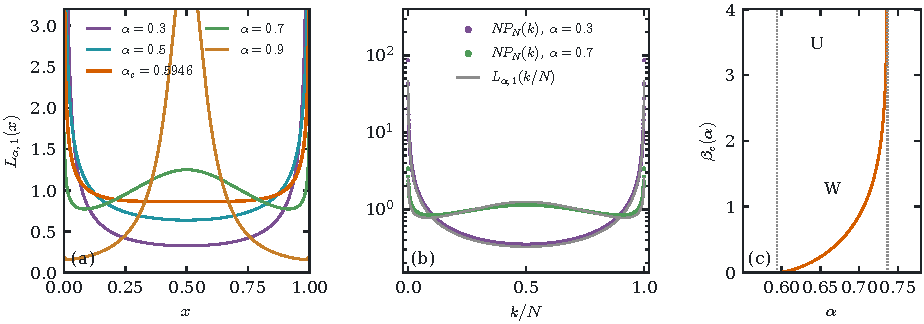
\includegraphics[width=\textwidth]{shape}
\caption{(a) The density $L_{\alpha,1}$ for $\alpha=0.3$, $0.5$, $\alpha_c$, $0.7$ and $0.9$.
At $\alpha_c$ the minimum at $1/2$ is flat to second order. (b) The exact law $NP_N(k)$ for
$N=2000$, the zeta law $f(n)\propto n^{-\alpha-1}$ for both signs and the fair start, with
$\alpha=0.3$ and $\alpha=0.7$, on a logarithmic scale, together with $L_{\alpha,1}(k/N)$. The
end values are of order $NT(N)$ and lie far above the density for $\alpha=0.3$. (c) The
threshold $\beta_c(\alpha)$ of Theorem~\ref{thm:shape} on $(\alpha_c,\alpha_1)$. Below the curve
$\La$ is W-shaped.
Section~\ref{sec:verify} describes the computations.}
\label{fig:shape}
\end{figure}

\begin{proof}
By~\eqref{eq:L-cosh}, $\La(x)=\frac{\sin\pi\alpha}\pi\phi(t)$ with $t=\log((1-x)/x)$ and
\[
 \phi(t)=\frac{1+\cosh t}{\cosh(\alpha t-\beta)+c}.
\]
The map $x\mapsto t$ is a decreasing diffeomorphism of $(0,1)$ onto $\R$, so the critical
points of $\La$ and of $\phi$ correspond, with the same type and the same order of
degeneracy. Put $s=\alpha t-\beta$ and $R(s)=\sinh s/(\cosh s+c)$, which is defined because
$\cosh s+c>0$. Then
\[
 \frac{\phi'(t)}{\phi(t)}=\tanh\frac t2-\alpha R(s)=:k(t).
\]
Since $R(s)\to\pm1$ as $s\to\pm\infty$, $k(t)\to\pm(1-\alpha)$ as $t\to\pm\infty$, so $\phi$
decreases near $-\infty$ and increases near $+\infty$. Hence the number of zeros of $k$ is
odd when they are simple, and if there are $3$ they are a minimum, a maximum and a minimum.

\emph{The function $H$.} The map $t\mapsto s$ is an increasing bijection. Let
$D=\{s:\alpha|R(s)|<1\}$. Off $D$ we have $|\alpha R(s)|\ge1>|\tanh(t/2)|$, so $k$ has no zero
there. On $D$ write $k(t)=\tanh A-\tanh B$ with $A=(s+\beta)/(2\alpha)$ and
$B=\operatorname{artanh}(\alpha R(s))$. Since $\tanh$ is increasing, $k$ has the sign of $A-B$,
that is of $\beta-H(s)$, where
\[
 H(s)=2\alpha\operatorname{artanh}(\alpha R(s))-s .
\]
So the critical points of $\La$ correspond bijectively to the solutions of $H(s)=\beta$ in
$D$. At a solution, $k'=\operatorname{sech}^2(A)(A'-B')=-\operatorname{sech}^2(A)H'(s)/(2\alpha)$ in the
variable $s$, and $\phi''=\phi k'$ there, so the critical point is nondegenerate exactly when
$H'(s)\ne0$.

\emph{The sign of $H'$.} We have $R'(s)=(1+c\cosh s)/(\cosh s+c)^2$, and with $w=\cosh s$ a
direct computation gives
\[
 2\alpha^2R'(s)-\bigl(1-\alpha^2R(s)^2\bigr)=-\frac{Q(w)}{(w+c)^2},\qquad
 Q(w)=(1-\alpha^2)(w-w_\minus)(w-w_\plus),
\]
where $w_\pm=-c\pm\alpha\sin(\pi\alpha)/\sqrt{1-\alpha^2}$ are the roots of
$(1-\alpha^2)w^2+2c(1-\alpha^2)w+c^2-\alpha^2$, whose discriminant is $4\alpha^2(1-\alpha^2)(1-c^2)$.
Since $H'(s)=[2\alpha^2R'-(1-\alpha^2R^2)]/(1-\alpha^2R^2)$ on $D$, and $w_\minus<1\le\cosh s$, we get
$H'(s)>0$ exactly when $\cosh s<w_\plus$ and $H'(s)<0$ exactly when $\cosh s>w_\plus$. With
$\sin\pi\alpha=2\sin(\pi\alpha/2)\cos(\pi\alpha/2)$ and $1+c=2\cos^2(\pi\alpha/2)$, the inequality
$w_\plus>1$ reads $\alpha\sin(\pi\alpha/2)>\cos(\pi\alpha/2)\sqrt{1-\alpha^2}$, and both sides are
nonnegative, so it is $\alpha^2>\cos^2(\pi\alpha/2)$, that is $\alpha>\alpha_c$.

\emph{The domain $D$.} The function $R$ is odd. If $c\ge0$, that is $\alpha\le1/2$, $R$ increases
on $[0,\infty)$ to the limit $1$, so $D=\R$. If $c<0$, $R$ increases on $[0,s_m]$ with
$\cosh s_m=-1/c$ to the value $R(s_m)=1/\sin\pi\alpha$, and then decreases to $1$. So $D=\R$ exactly
when $\alpha<\sin\pi\alpha$, that is $\alpha<\alpha_1$. For $\alpha\ge\alpha_1$ the set $D$ is $\R$
minus two closed intervals $\pm[s_1,s_2]$ around $\pm s_m$, which are single points when
$\alpha=\alpha_1$, and $H\to+\infty$ at both edges of $[s_1,s_2]$ and $H\to-\infty$ at both edges of
$[-s_2,-s_1]$, because $\alpha R\to1$ there from below. In every case $H$ is odd with $H(0)=0$,
and $H(s)\to\mp\infty$ as $s\to\pm\infty$, since $\alpha R\to\pm\alpha$ and $\operatorname{artanh}$ stays
bounded.

\emph{Counting.} Let $\alpha\le\alpha_c$. Then $D=\R$ and $H'<0$ except at $s=0$ when $\alpha=\alpha_c$,
so $H$ is a decreasing bijection of $\R$, and $H(s)=\beta$ has exactly one solution. It is
simple unless $s=0$ and $H'(0)=0$, that is $\alpha=\alpha_c$ and $\beta=0$. Let
$\alpha_c<\alpha<\alpha_1$. Then $D=\R$, $H'>0$ on $(-s_0,s_0)$ and $H'<0$ outside, so $H$ decreases
from $+\infty$ to a local minimum $-H(s_0)$ at $-s_0$, increases to the local maximum
$H(s_0)>H(0)=0$ at $s_0$, and decreases to $-\infty$. Hence $H(s)=\beta$ has $3$, $2$ or $1$
solutions according as $|\beta|<$, $=$ or $>H(s_0)$, all simple except the double one at
$\pm s_0$ in the case of equality. By the definition of $R$, $H(s_0)=\beta_c(\alpha)$
of~\eqref{eq:betac}, which is therefore finite and positive. Finally let $\alpha\ge\alpha_1$. On
$(0,s_1)$ the function $H$ rises from $0$ to $+\infty$, so $H'$ cannot be negative just below
$s_1$, which forces $s_0\ge s_1$ and $H'>0$ on $(-s_1,s_1)$. On $(s_2,\infty)$ it falls from
$+\infty$, which forces $s_0\le s_2$ and $H'<0$ there, and likewise on $(-\infty,-s_2)$. So each
of the three components of $D$ carries exactly one solution of $H=\beta$, all simple, for
every $\beta$. This proves (a) to (c).
\end{proof}

The monotonicity of $H$ is what closes the count. Descartes' rule for the exponential sum
that has the sign of $\phi'$ gives at most $3$ zeros only for $\alpha\le1/2$. As $\alpha$
increases to $\alpha_1$ the window $\beta_c$ opens to $\infty$, and at $b=0$ the dominated
regime of Section~\ref{sec:dominated} takes over. There the density~\eqref{eq:ratio-density}
of the ratio $Z_\minus/Z_\plus$ has an interior maximum exactly when $\alpha>\sin\pi\alpha$,
that is $\alpha>\alpha_1$, since the numerator of its logarithmic derivative in $r=y^\alpha$ is
$-(1+\alpha)r^2-2cr-(1-\alpha)$, which has a positive root exactly when $c<0$ and
$c^2>1-\alpha^2$. So the two shape thresholds meet at $\alpha_1$. Near $\alpha_c$ with $b=1$ the
two minima split off from $1/2$ like a pitchfork, at distance
$\frac14(3(2\alpha^2-1-\cos\pi\alpha)/(\alpha^2(1-\alpha^2)))^{1/2}(1+o(1))$ from $1/2$, which
follows from the expansion $\chi(t)=\chi(0+)+\frac13\alpha^2(1-\alpha^2)t^2(1+O(t^2))$ of the
function $\chi(t)=\cosh\alpha t+c-\alpha\sinh(\alpha t)\coth(t/2)$ that has the sign of $k$ for
$b=1$. At $\alpha=1/2$ and $b=1$ the theorem gives the arcsine density, with its minimum at
$1/2$.

\subsection{Difference forms of the renewal theorem}\label{sec:dsrt}

The end profiles are renewal mass functions. To compare neighbouring values of $P_N$ near an
end we need the differences of $u_\sgn$, and (DSRT$_\sgn$) asks that they have the size of
the derivative of $\frac{\sin\pi\alpha}\pi/(nT_\sgn(n))$. It holds for log-convex laws.

\begin{lemma}[the difference renewal theorem for log-convex laws]\label{lem:dsrt}
Let $f$ be a log-convex mass function on $\{1,2,\dots\}$ with $f(1)>0$ and a tail $T$ that is
regularly varying with index $-\alpha\in(-1,0)$. Then $f$ satisfies (LB) and (SRT), its renewal
mass function $u$ is strictly decreasing, and $u(j)-u(j+1)\sim(1-\alpha)u(j)/j$.
\end{lemma}

\begin{proof}
A log-convex $f$ that tends to $0$ is nonincreasing, so $f(n)\le2T(n/2)/n\le CT(n)/n$, which is
(LB), and Doney's theorem (Lemma~\ref{lem:cd}(iii)) gives (SRT), so $u$ is regularly varying
with index $\alpha-1$. By de Bruijn and Erd\H{o}s~\cite[Theorem~1]{debruijnerdos1953}, $u$ is
log-convex, so $r_j=u(j+1)/u(j)$ is nondecreasing, and $r_j<1$ because $u\to0$. For $\lambda>1$
and $i$ large put $j=\lfloor i/\lambda\rfloor$. Then
$\log u(i)-\log u(j)=\sum_{l=j}^{i-1}\log r_l$ lies between $(i-j)\log r_j$ and $(i-j)\log r_i$,
and tends to $(\alpha-1)\log\lambda$. Since $i-j\sim(\lambda-1)i/\lambda$, this gives
$\limsup_ii\log r_i\le(\alpha-1)\lambda\log\lambda/(\lambda-1)$, and applying the other inequality
with $i$ in place of $j$ gives $\liminf_jj\log r_j\ge(\alpha-1)\log\lambda/(\lambda-1)$. Let
$\lambda\downarrow1$. So $j\log r_j\to\alpha-1$, which is the claim.
\end{proof}

For Sibuya laws, $T(n)=\prod_{i<n}(1-\alpha/i)$, one has $r_j=(j+\alpha)/(j+1)$ exactly. The zeta
law $f(n)=n^{-\alpha-1}/\zeta(\alpha+1)$ is strictly log-convex. We do not know whether
(LR) and the first-difference condition $|f(n)-f(n+1)|=O(f(n)/n)$ imply (DSRT) when
$\alpha\le1/2$.

We also need the end profile of a prepared start. For an initial run $(\nu_\plus,\nu_\minus)$ with
$n\nu_\pm(n)\to0$, Theorem~\ref{thm:initial}(f) gives $P_N(N-j)/T_\plus(N)\to\kappa_\plus(j)$ for
$j\ge1$, with $\kappa_\plus$ as in~\eqref{eq:kappa-prep}, and we write
$\widetilde\kappa_\plus=(\widetilde\kappa_\plus(0),\kappa_\plus(1),\kappa_\plus(2),\dots)$ for the
profile with the end value $\widetilde\kappa_\plus(0)=\lim_NQ_\plus(N)/T_\plus(N)$, when this limit
exists in $[0,\infty]$. We say that the initial run satisfies (S) if
\begin{equation}\label{eq:S}\tag{S}
 |\nu_\sgn(n+1)-\nu_\sgn(n)|=o(n^{-2}),\qquad
 |\nu_\sgn(n+1)-2\nu_\sgn(n)+\nu_\sgn(n-1)|=o(n^{-3})
\end{equation}
for both signs, and the limits $\widetilde\kappa_\pm(0)$ exist. Fresh and fair starts satisfy (S)
under (LR) and (LD2), and so does every smooth regularly varying $\nu$, such as
$\nu(n)\propto n^{-1-\gamma}$ for any $\gamma>0$.

\begin{lemma}[the prepared profile]\label{lem:prep-profile}
Assume (BAL), (SPAN), (DSRT$_\minus$) and the first half of (S) for $\nu_\minus$. Then
$\kappa_\plus(j+1)-\kappa_\plus(j)=(1+o(1))(u_\minus(j+1)-u_\minus(j))$. In particular
$\widetilde\kappa_\plus$ is eventually strictly decreasing.
\end{lemma}

\begin{proof}
Write $u=u_\minus$, $\Delta u(i)=u(i+1)-u(i)$ and $\Delta u(0)=u(1)-1$. From~\eqref{eq:kappa-prep},
$\Delta\kappa_\plus(j)=\pi_\plus\Delta u(j)+\sum_{d\le j}\nu_\minus(d)\Delta u(j-d)+\nu_\minus(j+1)$. The
part $d\le j/2$ is $(\pi_\minus+o(1))\Delta u(j)$ by dominated convergence, since $\Delta u$ is
regularly varying by (DSRT$_\minus$). With $\sum_{i<j/2}\Delta u(i)=u(\lceil j/2\rceil)-1$, the rest
is $\sum_{0\le i<j/2}(\nu_\minus(j-i)-\nu_\minus(j+1))\Delta u(i)+\nu_\minus(j+1)u(\lceil j/2\rceil)$. With
$\delta_j=\sup_{n\in[j/2,j+1]}|\Delta\nu_\minus(n)|=o(j^{-2})$ and
$\sum_{i\le j}(i+1)|\Delta u(i)|\le Cju(j)$, this is at most $C\delta_jju(j)+o(1/j)u(j/2)=o(u(j)/j)$,
while $|\Delta u(j)|\sim(1-\alpha)u(j)/j$.
\end{proof}

\subsection{Sign changes of the discrete law}\label{sec:signs}

For a finite or infinite real sequence $(s_i)$ let $V(s)$ be the number of sign changes of
the sequence of its nonzero terms. The sign changes of $k\mapsto P_N(k+1)-P_N(k)$ are the
strict local extrema of $P_N$ when no two neighbouring values are equal.

\begin{theorem}[a lower bound on the sign changes]\label{thm:signs}
Assume (BAL), (SPAN) and (SRT$_\pm$), and let the initial run be such that
$NP_N(k)=\La(k/N)+o(1)$ uniformly on compact subsets of $(0,1)$ (for instance a fresh
start, or under (LB$_\pm$) any initial run with $n\nu_\pm(n)\to0$) and such that
$W^\pm_N=o(T_\pm(N))$. Assume that the limits $\widetilde\kappa_\pm(0)$ exist and are finite,
that $\widetilde\kappa_\pm(j+1)\ne\widetilde\kappa_\pm(j)$ for all $j\ge0$, and that
$\widetilde\kappa_\pm$ is strictly decreasing from some point on. Let
$\sigma_\pm=V((\widetilde\kappa_\pm(j+1)-\widetilde\kappa_\pm(j))_{j\ge0})$, and let $\sigma_L$ be the
number of critical points of $\La$, which is $1$ or $3$ by Theorem~\ref{thm:shape}, each of
them a strict local extremum. Then for all large $N$,
\[
 V\bigl((P_N(k+1)-P_N(k))_{0\le k<N}\bigr)\ge\sigma_L+\sigma_\plus+\sigma_\minus .
\]
\end{theorem}

\begin{proof}
If $(s_{i_l})$ is a subsequence of $(s_i)$, the differences of $(s_i)$ have at least as many
sign changes as the differences of $(s_{i_l})$, since each nonzero difference
$s_{i_{l+1}}-s_{i_l}$ is a sum of consecutive differences of $(s_i)$, one of which has its
sign. Let $c_1<\dots<c_s$ be the critical points of $\La$, $s=\sigma_L$. Since $\La\to\infty$ at
both ends, $\La$ decreases strictly on $(0,c_1]$ and increases strictly on $[c_s,1)$, and the
critical points alternate between strict minima and strict maxima, starting and ending with
a minimum. Choose $z_0\in(0,c_1)$ and $z_{s+1}\in(c_s,1)$. The differences of
$\La(z_0),\La(c_1),\dots,\La(c_s),\La(z_{s+1})$ have the signs $-,+,-,\dots,+$, with $s$ sign
changes. Choose $J$ such that $\widetilde\kappa_\plus$ and $\widetilde\kappa_\minus$ are strictly
decreasing on $[J-1,\infty)$, so $\widetilde\kappa_\pm(J)>0$. Consider the subsequence of
$(P_N(k))_{0\le k\le N}$ at the points
\[
 0,1,\dots,J,\ \lfloor z_0N\rfloor,\lfloor c_1N\rfloor,\dots,\lfloor c_sN\rfloor,\lfloor z_{s+1}N\rfloor,\ N-J,\dots,N .
\]
By Theorem~\ref{thm:initial}(f), its mirror, and the definition of $\widetilde\kappa_\pm(0)$,
$P_N(N-j)/T_\plus(N)\to\widetilde\kappa_\plus(j)$ and $P_N(j)/T_\minus(N)\to\widetilde\kappa_\minus(j)$ for
$0\le j\le J$. Since consecutive values of $\widetilde\kappa_\pm$ differ, for large $N$ the
differences at the two ends have the signs of the differences of $\widetilde\kappa_\pm$, with
$\sigma_\minus$ and $\sigma_\plus$ sign changes, and the differences next to $j=J$ have the sign
of $\widetilde\kappa_\pm(J)-\widetilde\kappa_\pm(J-1)<0$. In the bulk, $NP_N(\lfloor zN\rfloor)\to\La(z)$ at
each chosen point, so for large $N$ the bulk differences have the signs $-,+,\dots,+$ with $s$
sign changes. At the junctions, $P_N(J)\sim T_\minus(N)\widetilde\kappa_\minus(J)$ and
$P_N(N-J)\sim T_\plus(N)\widetilde\kappa_\plus(J)$, while the bulk values are $O(1/N)$ and
$NT_\pm(N)\to\infty$. So the difference from $P_N(J)$ to $P_N(\lfloor z_0N\rfloor)$ is negative and
the difference from $P_N(\lfloor z_{s+1}N\rfloor)$ to $P_N(N-J)$ is positive. Reading from left to
right, the last difference at the minus end, the junction and the first bulk difference are
all negative, and the last bulk difference, the junction and the first difference at the plus
end, which is $\sim T_\plus(N)(\widetilde\kappa_\plus(J-1)-\widetilde\kappa_\plus(J))$, are all positive.
So the junctions add no sign change, and the subsequence has $\sigma_\minus+s+\sigma_\plus$ sign
changes.
\end{proof}

\begin{example}[the fair start and the fresh start]\label{ex:counts}
Let both run laws be the zeta law, so $b=1$, and let the start be fair. Then
$Q_\pm(N)=\frac12T(N)$, so $\widetilde\kappa_\pm(0)=\frac12$, and~\eqref{eq:kappa-prep} gives
$\kappa_\pm(j)=\frac12u(j)+\frac12\sum_{d\le j}f(d)u(j-d)=u(j)$ for $j\ge1$. Since $u$ is strictly
decreasing by Lemma~\ref{lem:dsrt}, $\sigma_\pm=1$ if $u(1)=f(1)>\frac12$ and $\sigma_\pm=0$ if
$f(1)<\frac12$. Now $f(1)=1/\zeta(1+\alpha)$, and $\zeta(1.7)=2.054\ldots$ and
$\zeta(1.9)=1.750\ldots$. So Theorems~\ref{thm:signs} and~\ref{thm:shape} give at least $1$
sign change for $\alpha=0.3$ and $\alpha=0.5$, at least $3$ for $\alpha=0.7$, and at least
$3+1+1=5$ for $\alpha=0.9$. For a fresh plus start with different laws,
$\widetilde\kappa_\plus=(1,u_\minus(1),\dots)$ is strictly decreasing and
$\widetilde\kappa_\minus=(0,u_\plus(1),u_\plus(2),\dots)$ has one sign change, so the bound is
$\sigma_L+1$.
\end{example}

\subsection{The exact count}\label{sec:count}

In every case of Section~\ref{sec:verify} with a fresh, a fair or a smooth start, the computed
number of sign changes equals the lower bound of Theorem~\ref{thm:signs} for all large $N$.
Two difference statements turn the bound into an equality. We state them as hypotheses and
prove the count from them. For a fresh plus start put $D_N(j)=P_N(N-j-1)-P_N(N-j)$.
\begin{itemize}[leftmargin=4em,labelsep=0.8em]
\item[(L)] (The layer.) For every $\eta>0$ there are $\varepsilon>0$ and $J$ such that for all large
$N$ and $J\le j\le\varepsilon N$, $|D_N(j)-T_\plus(N)(u_\minus(j+1)-u_\minus(j))|\le\eta\,T_\plus(N)u_\minus(j)/j$,
and the mirror at the minus end.
\item[(B)] (The bulk.) Uniformly for $k/N$ in compact subsets of $(0,1)$,
$N^2(P_N(k+1)-P_N(k))\to\La'(k/N)$ and $N^3(P_N(k+1)-2P_N(k)+P_N(k-1))\to\La''(k/N)$.
\end{itemize}

\begin{proposition}[the exact count]\label{prop:count}
Assume (BAL), (SPAN), (LR), (LD2) and (DSRT$_\pm$), let the start be fresh or fair, assume
that $(\alpha,b)$ is not one of the degenerate pairs of Theorem~\ref{thm:shape}(c), and assume
(L) and (B). Let $J_\pm$ be such that $\widetilde\kappa_\pm$ is strictly decreasing on $[J_\pm,\infty)$,
assume $\widetilde\kappa_\pm(j+1)\ne\widetilde\kappa_\pm(j)$ for $j<J_\pm$, and let $M_\pm$ be the number
of local maxima of $\widetilde\kappa_\pm$. Let $m_L\in\{0,1\}$ be the number of interior maxima of
$\La$. Then for all large $N$, $P_N$ has exactly $M_\plus+M_\minus+m_L$ modes, $M_\plus$ of them
within $J_\plus$ of $N$, $M_\minus$ within $J_\minus$ of $0$, and the interior one, when
$m_L=1$, at $(x_{\max}+o(1))N$ with $x_{\max}$ the maximum of $\La$. Between the end blocks
lie exactly $1+m_L$ further local minima, at $(c+o(1))N$ for the minima $c$ of $\La$, and
no antimode in the layers. For strictly log-convex run laws $M_\plus=M_\minus=1$, so the count
is $2+m_L$.
\end{proposition}

\begin{proof}
We check the sign of $\Delta P_N(k)=P_N(k+1)-P_N(k)$ on five ranges. For $0\le j<J_\plus$,
Theorem~\ref{thm:initial}(f) gives $D_N(j)$ the sign of $\widetilde\kappa_\plus(j+1)-\widetilde\kappa_\plus(j)$,
since $n\nu_\pm(n)\to0$ for fresh and fair starts. For $J_\plus\le j\le\varepsilon N$, (L) and
(DSRT$_\minus$) give $D_N(j)<0$ once $\eta<1-\alpha$, so $P_N$ increases strictly toward the plus
end through the layer. By (B) and Theorem~\ref{thm:shape}, on $[\varepsilon N,(1-\varepsilon)N]$ the sign
of $\Delta P_N(k)$ is that of $\La'(k/N)$ away from the critical points, and near each critical
point $c$ the second difference has the sign of $\La''(c)\ne0$, so $\Delta P_N$ is strictly
monotone on a window of width $\delta N$ around $cN$ and changes sign exactly once there.
The minus end is the mirror. Taking $\varepsilon$ below the first critical point and above $1$
minus the last one makes the ranges overlap, and the signs agree on the overlaps, since
$\La'>0$ near $1$ and $D_N<0$ in the plus layer. Reading the signs of $\Delta P_N$ from $k=0$
to $k=N$, the pattern is that of the minus profile, then a block of negative signs, then the
bulk block, which is empty when $m_L=0$ and $(+)^{a}(-)^{b}$ when $m_L=1$, then a block of
positive signs, then the mirror of the plus profile. The modes are the changes from $+$ to
$-$, a leading $-$ and a trailing $+$, which gives $M_\minus+m_L+M_\plus$, and the minima are
the changes from $-$ to $+$, which are the minima of $\La$. For log-convex laws $u_\mp$ is
strictly decreasing with limit $0$, and the profiles $(1,u(1),\dots)$, $(0,u(1),\dots)$ and
$(\frac12,u(1),\dots)$ have one local maximum each, at $j=0$ or $j=1$ according as $u(1)$ is
below or above the end value, with no tie when $f(1)\ne\frac12$ for the fair start.
\end{proof}

What is proved toward (L) and (B). Lemma~\ref{lem:prep-profile} and
Theorem~\ref{thm:initial}(f) give the first range for every start with (S). For (L), the
decomposition of $D_N(j)$ by the fresh identity into four sums, as in the first-difference
theorem of~\cite[Section~6]{paperF}, reduces it to a difference form of Doney's local bound,
$|V_m(n-1)-V_m(n)|\le Cmf(n)/n$ for all $m\ge1$ and $n\ge a_m$ with $V_m=f^{*m}$, under (SPAN),
(LR) and the first-difference condition. This is the case $\alpha<1$ of the difference form
of the local big-jump theorem of~\cite[Section~6]{paperF}, with no centering, and we have not
written its proof. For (B),
the first-difference limit follows by taking a difference inside the proof of
Theorem~\ref{thm:local}, and the second-difference limit is the part that needs work: the range
of few runs contributes at the order $N^{-3}$ through the second differences of the convolution
powers. The computations of Section~\ref{sec:verify} agree with (L), (B) and the count in every
case.

\ifarxivbuild
\begin{remark}[a conjecture that fails]\label{rem:oscillating}
An earlier version of this paper conjectured that under the hypotheses of
Theorem~\ref{thm:signs}, (LB$_\pm$), the first-difference condition and strictly log-convex
run laws, the lower bound is an equality for all large $N$. It is not, because the hypotheses
of Theorem~\ref{thm:signs} put no smoothness on the initial run. Take Sibuya laws for both
signs and an initial plus run with $\nu_\plus(n)=c\,n^{-1-\alpha}(1+0.9(-1)^n)$ for $n\ge2$ and the
rest of the mass at $d=1$. Then $n\nu_\plus(n)\to0$, $Q_\plus(N)/T(N)$ converges, and $\kappa_\minus$
is eventually strictly decreasing, so every hypothesis holds. The alternating part of
$\nu_\plus$ enters $P_N(k)$ through $\nu_\plus(k)T_\minus(N-k)$ and the near-diagonal terms, with
an amplitude of order $N^{-1-2\alpha}$ that does not cancel, and it beats the slope of
$\La(k/N)/N$ near every critical point. For $\alpha=0.7$ the exact law has $31$, $35$, $50$ and
$62$ modes at $N=500$, $1000$, $2000$ and $3000$, and for $\alpha=0.3$ with
$\nu_\plus(n)=c(n^{-1-\alpha}+0.3(-1)^nn^{\alpha-2})$ it has $54$, $110$, $223$ and $338$. The
condition (S) excludes these starts, and the count of Proposition~\ref{prop:count} holds
for them in no form. At the degenerate point $\alpha=\alpha_c$, $b=1$, the count depends on the
law: with the fair start the Sibuya law has $3$ modes and the zeta law $2$ at every computed
$N\le3000$, so the nondegeneracy hypothesis cannot be dropped.
\end{remark}
\fi
